%% アブスト
\documentclass[a4j,twoside]{jarticle}
\usepackage[dvipdfmx]{graphicx}
\usepackage{thesis_abst}
\usepackage{cite}
\usepackage{slashbox}
%%マージンはプリンタによって変更
\addtolength{\oddsidemargin}{0mm}
\addtolength{\evensidemargin}{0mm}

%%baselinestretchを変更すると上部枠の大きさが変わるのでおすすめしない
\renewcommand{\baselinestretch}{1}

\種別{卒 業} %{卒 業}または{修 士} 間に半角スペースを入れる
\学籍番号{28114006}
\氏名{石島 侑弥}
%%\英語氏名{} %未使用
\研究室{李}
\分野{メディア}
\題目{対話状態追跡における対話行為タグを用いた重要対話履歴抽出}
 % 途中で改行 "\\" を挿入可
\年度{2019} % !=年 発表は2月です

\begin{document}              %この行を消してはいけない
\twocolumn[\vspace*{9mm}]     %この行を消してはいけない
\begin{論文概要}              %この行を消してはいけない
  \setcounter{page}{1}          %表(左綴じ)は1、裏(右綴じ)は2を指定
  \setlength{\baselineskip}{3.7mm}
  \newcommand{\bm}[1]{\mbox{\boldmath$#1$}}
  \def\argmax{\mathop{\rm argmax}}
  \def\tr{\mathop{\rm tr}}
  \def\sp{~~~~~}
%%%%%%% ここからアブスト本体 %%%%%%%
\vspace{-2mm}
\section{はじめに}
対話システムは,ユーザが持つ特定の目的を対話によって達成するタスク指向型対話システムと,対話そのものを目的とする雑談対話システムに大別される.対話状態追跡とは,ユーザの目的や要求を対話状態に反映し,適切に維持あるいは更新するタスクであり,タスク指向型対話システムの重要な要素である.
\par
近年では,深層学習を用いた End-to-End 型の対話状態追跡モデルが高い性能を示しており,発話文から対話状態を直接出力することが可能となった\cite{nbt,e2e}.発話文を入力とするにあたり,対話履歴が対話の流れを捉えるために用いられている.
従来研究では対話履歴として直近の数発話を入力とするが,計算量を抑えるために多くの発話文を入力しないことが多く,対話状態の推定に貢献する文が含まれないことがある.
\par
本研究では,システムの発話意図を示す対話行為タグを用いて,長い対話履歴の中から対話状態追跡に重要だと思われるシステム発話を抽出する手法を提案する.対話行為タグによって各システム発話を意図ごとに分類し,特に状態に影響を与える発話を選択的に抜き出すことで,計算量を抑えつつ長い対話履歴を考慮することが可能であると期待できる.
\par
対話システムの国際コンペティションであるDialogue System Technology Challenge 8 Track4 Dialogue State Tracking (DSTC8-Track4) \cite{dstc8} において,対話状態追跡の  SGD データセットとベースラインモデルが公開されている.そのデータセットとモデルを用いて実験を行い従来手法と提案手法の比較を行う.

\vspace{-2mm}
\section{DSTC8-Track4}
\begin{figure}[htb]
  \centering
  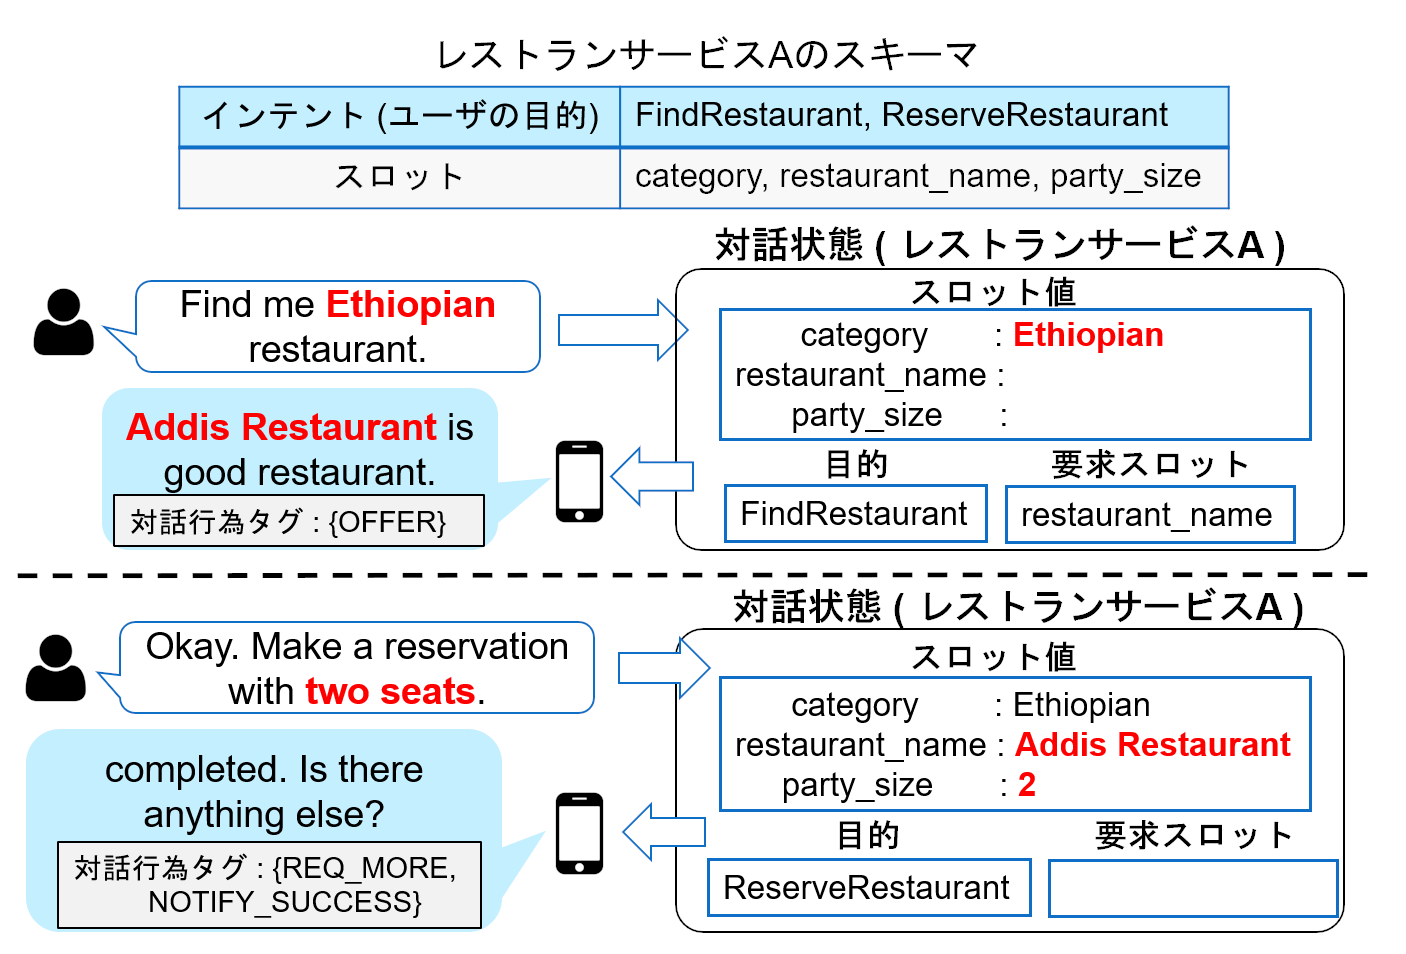
\includegraphics[width=7.9cm]{task.eps}
  \caption{DSTC8-Track4 のイメージ図}
  \label{fig:task}
\end{figure}
DSTC8-Track4 は,新サービスや新ドメインへの対応を再学習なしで可能にする対話状態追跡モデルを作成することを目的としたタスクである.本タスクのイメージ図を図\ref{fig:task}に示す.
\par
SGD データセットでは,レストラン案内や交通案内などのドメインごとに複数のサービスが存在する.そして,サービスごとにサービスを定義する枠組みであるスキーマが与えられ,対話状態を定義するために用いられる.スロットはユーザの要求を示すための属性で,インテントは目的である.対話状態は,ユーザの要求をスロットと値の組によって表すスロット値と,インテント,ユーザが値を要求しているスロットのリストである要求スロットで構成される.そして,ユーザが発話した際にそれまでの対話中に存在する情報を捉えて対話状態に反映する.また,システム発話には発話の意図を示す対話行為タグ,スキーマにはスロットと目的の意味をシステムが理解するための説明文が付与されている.そのため,入力として対話文,スキーマ,対話行為を用いて,対話状態を出力する.

\vspace{-2mm}
\section{対話行為タグを用いた重要対話履歴抽出}
%\begin{figure}[htb]
  %\centering
  %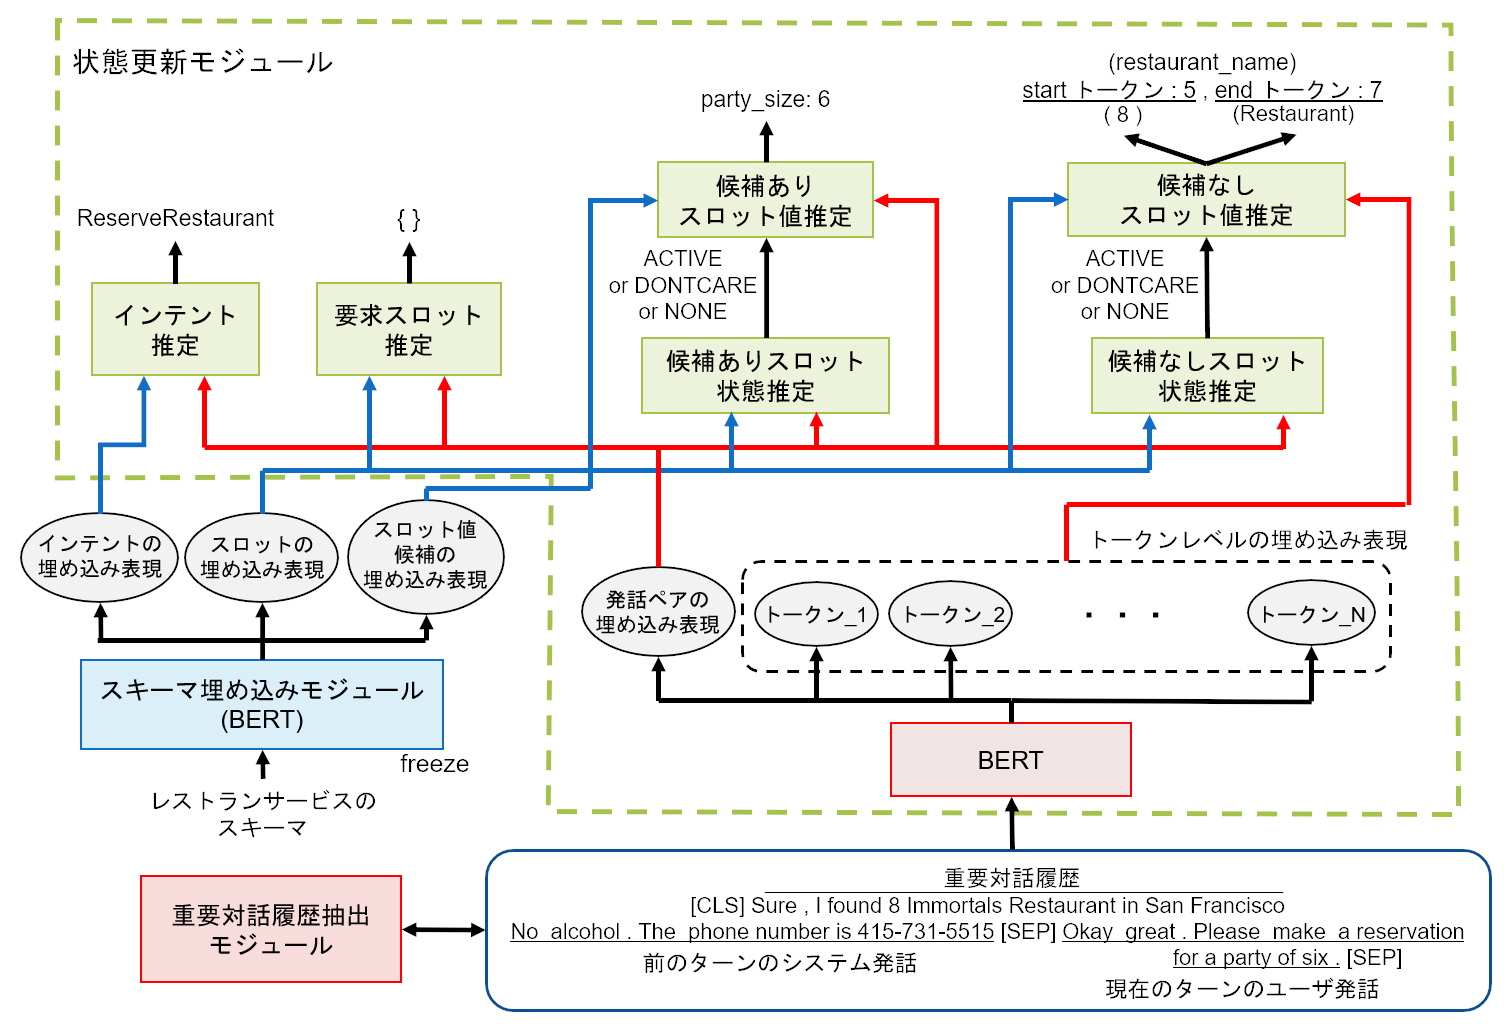
\includegraphics[width=7.9cm]{teian2.eps}
  %\caption{提案モデル}
  %\label{fig:teian}
%\end{figure}
重要対話履歴とは,対話状態に反映されるスロット値を持つなど対話状態の推定に貢献する発話を指す.
提案モデルではDSTC8-Track4で提供されているベースラインモデルに重要対話履歴抽出モジュールを加える.このモジュールは,入力文中にある前のターンのシステム発話が特定の対話行為タグを持つ場合に,その発話を保持する.既に発話を保持している場合は,新しい発話に更新する.そして,元々保持されていた発話を重要対話履歴として入力に加える.入力は,重要対話履歴,前のターンのシステム発話,現在のターンのユーザ発話の3発話とする.
\vspace{-2mm}
\section{評価実験}

DSTC8-Track4 では,目的の推定精度を示す Active Intent Accuracy(AIA),要求スロットの推定精度を示す Requested Slots F1(RSF1),スロット値の推定精度を示す Average Goal Accuracy(AGA) と Joint Goal Accuracy(JGA) を用いる.本実験ではこれらの指標に加え,学習時間も評価に用いる. \par
\begin{table}[h]
  \begin{center}
    \caption{提案手法と従来手法の比較}
    \label{tab:res}
    \begin{tabular}{|c|c|c|c|} \hline
      & AIA & RSF1 & AGA \\ \hline
      \begin{tabular}{c}
        従来手法\\(直近4発話入力)
      \end{tabular} & 0.974 & 0.948 & 0.844 \\ \hline
      \begin{tabular}{c}
        提案手法\\(OFFER)
      \end{tabular} & 0.946 & 0.947 & 0.845 \\ \hline \hline
      & JGA & \multicolumn{2}{c|}{学習時間} \\ \hline
    \begin{tabular}{c}
      従来手法\\(直近4発話入力)
    \end{tabular} & 0.553 & \multicolumn{2}{c|}{26.3(h)} \\ \hline
    \begin{tabular}{c}
      提案手法\\(OFFER)
    \end{tabular} & 0.565 & \multicolumn{2}{c|}{20.7(h)} \\ \hline
  \end{tabular}
  \end{center}
\end{table}
提案手法では,ユーザにスロット値を提案する“OFFER”タグが事前に行った実験で最良の結果を示したため,それを用いている.また,従来手法は直近4発話入力としている.これら2つを比較した結果,JGAは提案手法の方が 1.2\% 高い結果を示し,学習時間も削減している.ゆえに,提案手法はモデルの学習時間を減らすのと同時に,性能を向上させることが可能であるといえる.
\vspace{-2mm}
\section{むすび}
本研究では,対話状態追跡における対話履歴の使い方として,システムの対話行為タグを用いて重要な対話履歴を抽出する手法を提案した.今回の手法は人間が選択的にどの対話行為タグを持つ発話に注目するかを決めている.この手法でも性能は向上するが,機械側で対話履歴中のどの発話に注目すべきかを推定可能な対話状態追跡モデルを検討したい.
\footnotesize

%%%%%%
\vspace{-1mm}
\begin{thebibliography}{99}
%\bibitem{bert}
%Jacob Devlin et al. BERT:Pre-training of deep bidirectional transformers for language understanding. InProceedings of the 2019 Conference of the North American Chapter of the Association for Computational Linguistics: Human Language Technologies, Volume 1(Long and Short Papers), pages 4171--4186, 2019.
\bibitem{nbt}
%Nikola Mrk{\v{s}}i{\'c}, Diarmuid {\'O} S{\'e}aghdha Wen Tsung-Hsien, Blaise Thomson, and Steve Young. Neural Belief Tracker: Data-Driven Dialogue State Tracking. arXiv preprint arXiv:1606.03777. 2019.
Nikola Mrk{\v{s}}i{\'c} et al. Neural Belief Tracker: Data-Driven Dialogue State Tracking. arXiv preprint arXiv:1606.03777. 2017.

\bibitem{e2e}
Bing Liu and Ian Lane. An End-to-End Trainable Neural Network Model with Belief Tracking for Task-Oriented Dialog. In Proceedings of Interspeech 2017, pages 2506--2510, 2017.

\bibitem{dstc8}
Seokhwan Kim et al. The eighth dialog system technology challenge. InThird NeurIPS workshop on Conversational AI:“Today’s Practice and Tomorrow’s Potential”, 2019.
\end{thebibliography}

%%%%%% 以下の行は消さないこと %%%%%%%
\clearpage                       %この行を消すと最終ページの枠線消滅の危機
\end{論文概要}                   %この行を消してはいけない
\end{document}                   %この行を消してはいけない
